%!TEX TS-program = lualatex

\documentclass[12pt]{article}
\usepackage[utf8]{inputenc}
\usepackage[T1]{fontenc}

%!TEX TS-program = lualatex
\usepackage{tikz}
\usepackage{calc}
\usepackage{booktabs}
\usepackage[base]{babel}
\usepackage{hyperref}
\usepackage{graphicx}
\usepackage{wrapfig}
\usepackage{lipsum}
\usepackage[toc]{appendix}
\usepackage{xcolor}

% colors
\definecolor{color1}{HTML}{000060}
%\definecolor{color1}{HTML}{8C260F}
\definecolor{color2}{HTML}{333333}
\definecolor{lightgray}{gray}{0.9}

% fonts
\usepackage{fontspec}
\usepackage{unicode-math}
\defaultfontfeatures{Ligatures=TeX}
\setmainfont[Ligatures=TeX]{Candara}
%\setmathfont{XITS Math}
\newfontfamily\headingfont[]{Candara}
%%%

\usepackage{geometry}
\geometry{a4paper,
      hmargin=20mm,vmargin=20mm,
      head=0ex,foot=3ex}

\linespread{1.3}

\usepackage[hang]{caption}
\DeclareCaptionFormat{upper}{#1#2\uppercase{#3}\par}
\captionsetup{labelfont={bf,color=color2},textfont={normalsize,color=color2},format = upper,figurename=FIGURE,tablename=TABLE}

%%% fancy sections
\usepackage{titlesec}
%\titleformat{\chapter}{\headingfont\LARGE\bfseries\scshape\color{color1}}{\thechapter}{1em}{}[\titlerule]
\titleformat{\section}{\color{color1}\headingfont\Large\bfseries\uppercase}{\thesection}{1em}{}[\titlerule]
\titleformat{\subsection}{\color{color1}\headingfont\large\bfseries\uppercase}{\thesubsection}{1em}{}
\titleformat{\subsubsection}{\color{color1}\headingfont\bfseries\uppercase}{\thesubsubsection}{1em}{}
%%%

% head and foot
\usepackage{fancyhdr}
\pagestyle{fancy}
\lhead{}
\chead{}
\makeatletter
\rhead{\color{color2}\@date}
\makeatother
\newlength{\myheight}
\setlength{\headheight}{15pt}
\renewcommand\headrulewidth{0pt}
\renewcommand\footrulewidth{0pt}

%%% picture on cover page
\usepackage{eso-pic}
\newcommand\BackgroundPic{%
      \put(0,0){%
            \parbox[b][\paperheight]{\paperwidth}{%
                  \vfill
                  \centering
                  
\includegraphics[width=\paperwidth,height=\paperheight,%
                        keepaspectratio]{cover}%
                  \vfill
            }}}
%%%
% custom titlepage
\makeatletter
\renewcommand{\maketitle}{
      \thispagestyle{empty}
      \AddToShipoutPicture*{\BackgroundPic}
      \ClearShipoutPicture
      %
      \phantom{a}
      \vfill
      \phantom{a}\hfill
      \begin{tabular}[c]{@{}p{0.7\textwidth}@{}}
            \color{white}\headingfont\LARGE\@title  \\[1em]
            \color{white}\headingfont\Large\@author \\[2em]
      \end{tabular}
      %
      \clearpage
}
\makeatother
%%%


%%% fancy boxes
\usepackage{tcolorbox}
\usepackage{wrapfig}
\def\fullboxbegin{
      \bigskip
      \begin{tcolorbox}[colback=color1,colframe=color1,coltext=white,arc=0mm,boxrule=0pt]
            }
            \def\fullboxend{\end{tcolorbox}\medskip}
%
\def\leftboxbegin{
      \begin{wrapfigure}{l}{0.5\textwidth}
            \begin{tcolorbox}[colback=color1,colframe=color1,coltext=white,arc=0mm,boxrule=0pt]
                  }
                  \def\leftboxend{
            \end{tcolorbox}
      \end{wrapfigure}
}
%
\def\rightboxbegin{
      \begin{wrapfigure}{r}{0.5\textwidth}
            \begin{tcolorbox}[colback=color1,colframe=color1,coltext=white,arc=0mm,boxrule=0pt]
                  }
                  \def\rightboxend{
            \end{tcolorbox}
      \end{wrapfigure}
}
%
\newcounter{frames}
\def\frameboxbegin#1{
      \bigskip
      \refstepcounter{frames}
      \begin{tcolorbox}[colback=white,colframe=color1,arc=0mm,title={\MakeUppercase{\textbf{Frame \arabic{frames}}: #1}}]
            }
            \def\frameboxend{
      \end{tcolorbox}
}
%%%


%%%%%%%%%%%%%%%
% Title Page
\title{ADQ14 Hard X-Ray Monitor}
\author{Wojciech Walewski \newline DMCS}
\date{\today}
%%%%%%%%%%%%%%%

\begin{document}
\maketitle

\tableofcontents
\clearpage

\section{Introduction}

	\subsection{Document structure}
	This document describes the functionality of a firmware package developed for the ADQ14 digitizer.
	The solution implements a real time Pulse Height Analyzer for exponential pulses, intended
	for use in Hard X-Ray Monitors. The Pulse Height Analyzer firmware is built on top of the SPDevices ADQ14 DevKit.
	Initial chapters of this paper go over the digitizer board itself, highlighting its features and limitations.
	The custom firmware solution is built on top of a development kit provided by SPDevices with ADQ14.
	\newpage
\section{ADQ14}
	\subsection{}

\section{SPDevices DevKit}
	The custom spectroscopy firmware is built on top of a development kit provided with the digitizer board.
	The base system is referred to as the DevKit by the manufacturer. A full documentation of the DevKit can
	be downloaded from the \href{https://www.spdevices.com/documents/user-guides/24-adq14-development-kit}{manufacturer's website}.
	An offline copy is included with the firmware source code in the \verb|documentation| folder.
	\subsection{The concept of User Logic}
		\begin{wrapfigure}[14]{r}{0.28\textwidth}
			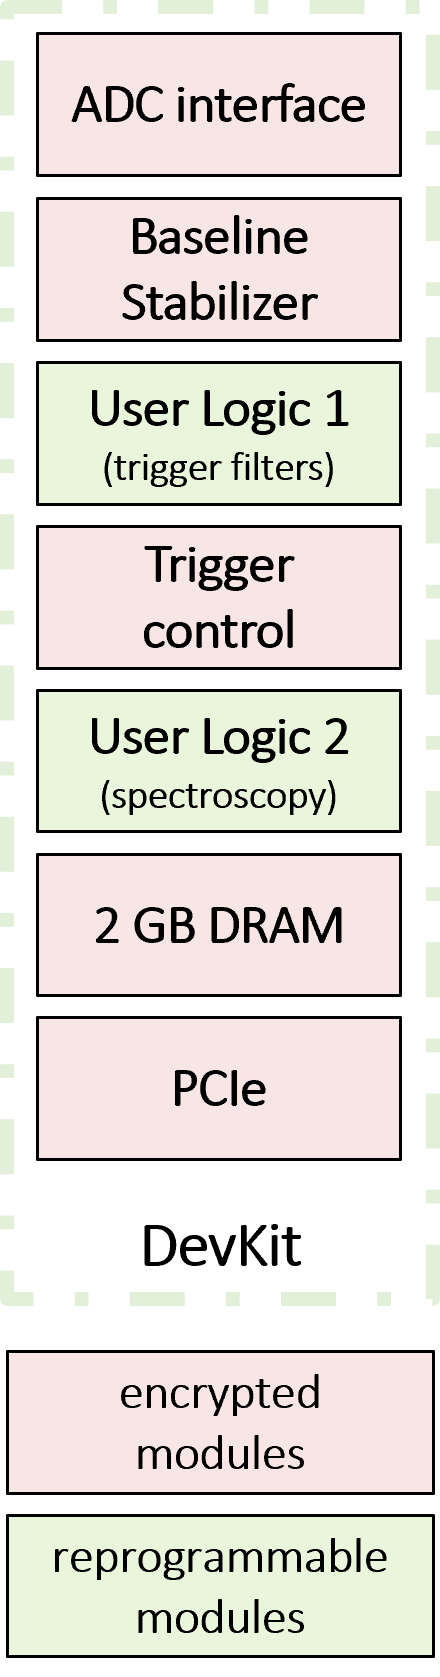
\includegraphics[width=0.25\textwidth]{img/devkit_ul.png}
			\caption{DevKit overview}\label{wrap-fig:devkit_ul}
		\end{wrapfigure}
		The modules provided with the DevKit control the Analog Digital Converter, triggering,
		packeting, the DRAM data queue and the PCIe interface. The subsystems responsible for these
		parts of the pipeline are provided in the form of encrypted IP cores and cannot be modified.
		Two modifiable modules, referred to as User Logic 1 and 2, are exposed in between,
		enabling the use of entirely custom algorithms at two points in the data flow.
		User Logic 1 is placed right before the trigger control, enabling the use of
		detection or smoothing filters with the digitizer's level trigger feature.
		User Logic 2 allows for modifications being placed right before the individual consecutive
		samples are packed into records, assigned metadata and queued in the DRAM for transmission to the
		host computer. The DevKit structure, with the placement of the User Logic modules highlighted in gold,
		is shown in \autoref{wrap-fig:devkit_ul}. Both modules are described in greater detail in the next chapters.
		\par
		\newpage
	\subsection{Samples in the FPGA}
		\begin{figure}[!h]
			\centering
			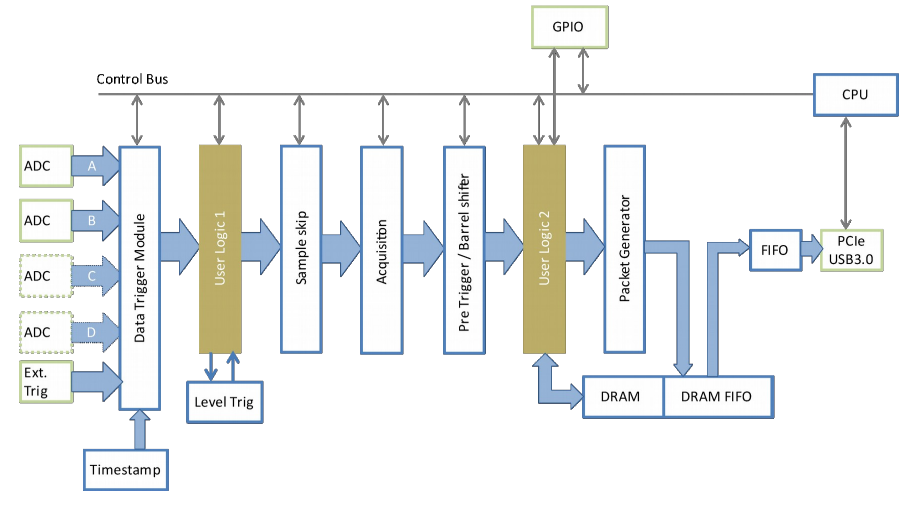
\includegraphics[width=0.83\textwidth]{img/devkit_dataflow.png}
			\caption{Primary data flow in the FPGA}\label{fig:devkit_dataflow}
		\end{figure}
		The digitizer's ADC is capable of sampling the signal at a rate up to 1 GS/s or 1 GHz.
		The FPGA is clocked at 250 MHz, resulting in a parallel design where each channel produces
		4 new consecutive samples for the FPGA on each clock cycle. The ADCs produce 14-bit samples.
		The raw signal is however subject to a digitial gain and shift.
		Two additional fractional bits are appended to the 14-bit samples before calculations.
		Two configurations are factored in the gain and shift calculations. The board comes preconfigured
		with a factory calibration that is always applied. A second configuration is made available to
		the users and can be freely modified from base values to apply custom digital signal shift or change the gain.
	\subsection{Data flow in User Logic 1}
		After the digital gain and shift, the 16-bit samples are packed into a data bus and made available at
		the User Logic 1 module. This component is located before the level trigger. By default the raw sample data
		is passed on to the triggering module unchanged. If the device trigger mode is set to the level trigger,
		digital filters can be implemented in User Logic 1 to modify the trigger behaviour. In initial testing
		a configurable moving average smoothing filter was placed in this module to reduce the influence of noise.
		At one point a boxcar and a trapezoidal filters were successfully implemented for pulse detection.
		These filtering modules were created in an abstract manner and can be combined to modify the level trigger
		behaviour to a desired shape and signal-to-noise ratio.
		\par
		The samples that are passed to the level trigger module can differ from those that are sent further
		down the processing pipeline, meaning that it is possible to trigger on appropriately filtered data,
		while still storing unmodified samples at the host PC. The current version of the firmware does not
		perform any filtering in this part of the firmware. All spectroscopy logic has been moved to User Logic 2,
		however the filter modules remain usable and can be reintroduced if the need appears.
	\subsection{Data flow in User Logic 2}
		User Logic 2 deals with data that has passed through User Logic 1, decimation and shifting to accomodate
		for pretrigger (horizontal shift). User Logic 2 is responsible for tagging the start and end of a single
		acquisition window (record). Further DevKit modules can then then pack and queue the records for transmission.
		User Logic 2 also inserts header data containing the metadata. The record length is fixed by default and set
		\par
		All spectroscopy logic in the current firmware revision is contained within User Logic 2. 
		\autoref{appendix:user_logic} contains a detailed description of the input and output signals 
		available in the User Logic modules, mostly useful for firmware developers.
	\subsection{Data paths in the FPGA}
		Records built of the 16-bit samples, together with the metadata are initially stored in the digitizer's
		internal DRAM. This memory forms a FIFO queue, that is periodically transferred over to the host PC. The 
		ADQ14's RAM has a capacity of 2 GB. With two bytes per sample up to a billion samples can be queued
		for data transfer before overflow leads to data loss. With up to a billion samples being generated
		every second for every active channel, this memory must be efficiently transferred.
		Two data paths exist within the firmware for exchanging data with the host PC.
		\subsubsection{DMA}
		After being packed in records and queued in the digitizer's DRAM, the acquired samples are sent
		using Direct Memory Access. This path makes it possible to write data directly to the host PC's RAM, 
		without the need of CPU involvment. Naturally, the host PC's RAM is not unlimited, 
		so the data must be processed (e.g. saved to a hard drive) at a rate comparable to the DMA transfers.
		DMA is a one-way path, so data can be transferred from the digitizer to the host PC,
		but not the other way around.
		Any data can be inserted in place of the samples for each channel to leverage the fast data path. 
		The custom Pulse Height Analyzer relies on this fact to periodically transfer computed spectras.
		\subsubsection{User Registers}
		A substantially slower two-way data path is available through the user registers (top data bus on \autoref{fig:devkit_dataflow}). Both User Logic modules
		implement a small individually addressable memory block, that can be written to or read from by both 
		the host PC and the FPGA. The memory structure contains 32-bit integers. $2^{14}$ addressable words
		are available in User Logic 1, and $2^{19}$ in User Logic 2. First 4 positions in both modules are reserved 
		for internal use by the DevKit and cannot be modified in the custom firmware. The custom PHA firmware
		relies on User Registers primarily for transferring configuration settings to the FPGA.
		The current version of the firmware also enables spectra transfer through this data path for testing purposes.
	\subsection{Bypassing User Logic}


\section{Custom Firmware}
\subsection{Core Firmware Functionality}
The firmware spectroscopy solution consists of four primary subsystems:
\begin{itemize}
	\item Pulse Detection Module
	\item Pulse Shaping Module
	\item Pulse Sampler
	\item Spectrum Storage and Transfer
\end{itemize}
\subsection{Pulse Detection Module}
\subsection{Pulse Shaping Module}
\subsection{Pulse Sampler}
\subsection{Spectrum Storage and Transfer}
\section{Second section}

\fullboxbegin
\lipsum[1]
\fullboxend

\lipsum[1]

\subsection{First subsection}
\lipsum[1]

\leftboxbegin
Lorem ipsum dolor sit amet, consectetuer adipiscing elit. Ut purus elit, vestibulum ut, placerat ac, adipiscing vitae, felis. Curabitur dictum gravida mauris. Nam arcu libero, nonummy eget, consectetuer id, vulputate a, magna. Donec vehicula augue eu neque.
\leftboxend

\lipsum[1-2]

\rightboxbegin
\begin{itemize}
	\item Lorem ipsum
	\item Lorem ipsum
\end{itemize}
\rightboxend
\lipsum[1]
\begin{table}[!h]
	\centering
	\caption{Sample table.}
	\begin{tabular}{cccc}
		\toprule
		Value 1 & Value 2 & Value 3 & Value 4 \\
		\midrule
		odd     & odd     & odd     & 1.00    \\
		even    & even    & even    & 1.00    \\
		odd     & odd     & odd     & 1.00    \\
		even    & even    & even    & 1.00    \\
		\bottomrule
	\end{tabular}
\end{table}

\lipsum[1]

\frameboxbegin{Sample frame}
\lipsum[1]
\frameboxend

\appendix
\section{User Logic Data Bus}\label{appendix:user_logic}
\subsection{User Logic 1}\label{appendix:user_logic_1}
\lipsum[1]
\subsection{User Logic 2}\label{appendix:user_logic_2}
\lipsum[1]
\end{document}
